\documentclass[hyperref={breaklinks=true},fleqn,mathserif]{beamer}

\usepackage{graphicx}
\usepackage{booktabs}
\usepackage{array}
\usepackage{amssymb}
\usepackage{listings}
\usepackage{tikz}
\usetikzlibrary{arrows.meta,positioning,fit,calc,shapes.geometric}

%%%%%%%%%%%%%%%%%%%%%%%%%%%%%%%%%%%%%%%%%%%%%%%%%%%%%%%%%%%%%%%%%%%%%%%%%%%%%%%%
\usepackage[utf8x]{inputenc}
\usepackage[L7x]{fontenc}
\usepackage[english,lithuanian]{babel}
%%%%%%%%%%%%%%%%%%%%%%%%%%%%%%%%%%%%%%%%%%%%%%%%%%%%%%%%%%%%%%%%%%%%%%%%%%%%%%%%

\usetheme{Warsaw}
\setbeamertemplate{navigation symbols}{}
\setbeamersize{text margin left=1em,text margin right=1em}

\title[Dinaminė žmogžudysčių duomenų bazė]{Dinaminė žmogžudysčių duomenų bazė}
\subtitle{Rezultatai, algoritmai ir tolesni planai}
\author[\textit{et al.}]{\textbf{Paulius Jankauskas}, Tomas Sarafin ir \\ Justas Daugirdas}
\institute{Vilniaus universitetas \\ Matematikos ir informatikos fakultetas }
\date{2026 m. spalio 28 d.}

\defbeamertemplate*{footline}{shadow theme}
{%
    \leavevmode%
    \hbox{%
        \begin{beamercolorbox}[wd=.5\paperwidth,ht=2.5ex,dp=1.125ex,leftskip=.3cm plus1fil,rightskip=.3cm]{author in head/foot}%
            \usebeamerfont{author in head/foot}\insertframenumber\,/\,\inserttotalframenumber\hfill\insertshortauthor
        \end{beamercolorbox}%
        \begin{beamercolorbox}[wd=.5\paperwidth,ht=2.5ex,dp=1.125ex,leftskip=.3cm,rightskip=.3cm plus1fil]{title in head/foot}%
            \usebeamerfont{title in head/foot}\insertshorttitle%
        \end{beamercolorbox}%
    }%
    \vskip0pt%
}

% Code listings (code itself is ASCII only). Computer Modern has no L7x
% typewriter font, so use Latin Modern's for code and \texttt.
\renewcommand{\ttdefault}{lmtt}
\definecolor{codebg}{RGB}{245,245,250}
\definecolor{codekw}{RGB}{38,38,134}
\definecolor{codecm}{RGB}{110,110,110}
\definecolor{codestr}{RGB}{150,40,40}
\definecolor{termbg}{RGB}{30,32,36}
\definecolor{termfg}{RGB}{225,225,225}
\definecolor{termhi}{RGB}{120,210,120}
\definecolor{termerr}{RGB}{240,120,110}
\lstset{
    language=Python,
    basicstyle=\ttfamily\scriptsize,
    keywordstyle=\color{codekw}\bfseries,
    commentstyle=\color{codecm}\itshape,
    stringstyle=\color{codestr},
    backgroundcolor=\color{codebg},
    frame=single, rulecolor=\color{codebg},
    columns=fullflexible, keepspaces=true,
    showstringspaces=false, breaklines=true,
    xleftmargin=2pt, xrightmargin=2pt,
}
\lstdefinestyle{sql}{language=SQL, morekeywords={ROLE,LOGIN,NOINHERIT,LIMIT,REVOKE}}
\lstdefinestyle{term}{
    language={}, basicstyle=\ttfamily\tiny\color{termfg},
    backgroundcolor=\color{termbg}, rulecolor=\color{termbg},
    columns=fullflexible, breaklines=false,
    emph={detective}, emphstyle=\color{termhi}\bfseries,
    emph={[2]rejected,ERROR,wrong}, emphstyle={[2]\color{termerr}\bfseries},
}

% TikZ styles
\tikzset{
    box/.style={draw=structure, fill=structure!8, rounded corners=3pt, align=center,
                font=\scriptsize, inner sep=4pt, minimum height=8mm},
    hot/.style={box, draw=red!70!black, fill=red!8},
    good/.style={box, draw=green!45!black, fill=green!8},
    arr/.style={-{Latex[length=2mm]}, thick, structure},
    lbl/.style={font=\tiny, fill=white, inner sep=1pt},
    tbl/.style={draw=structure, fill=white, rounded corners=2pt, align=left,
                font=\tiny, execute at begin node={\hyphenpenalty=10000\relax},
                inner sep=2.5pt, text width=32.5mm},
    fk/.style={-{Latex[length=1.6mm]}, structure!70},
}
\newcommand{\tname}[1]{\textbf{\scriptsize #1}\\[1pt]}
\newcommand{\yes}{\textcolor{green!50!black}{$\checkmark$}}
\newcommand{\no}{\textcolor{red!70!black}{$\times$}}

\begin{document}

\frame[plain]{\titlepage}


% ============================================================
% KAS PASIKEITĖ NUO SEMINARO 3
% ============================================================
\begin{frame}{Kas pasikeitė nuo Seminaro 3}

\begin{columns}[T]
\begin{column}{0.47\textwidth}
\begin{alertblock}{Seminaras 3}
\footnotesize
\begin{itemize}
    \setlength{\itemsep}{2pt}
    \item Tik terminalo programa.
    \item 500 asmenų, \textbf{1955} įrašai bazėje.
    \item Žudikas randamas \textbf{viena JOIN užklausa}.
    \item Žudiko apklausoje buvo prisipažinimas.
\end{itemize}
\end{alertblock}
\end{column}

\begin{column}{0.51\textwidth}
\begin{exampleblock}{Dabar}
\footnotesize
\begin{itemize}
    \setlength{\itemsep}{2pt}
    \item \textbf{Web sąsaja} („policijos įrašų sistema“) ir terminalas.
    \item Bazė sumažinta iki \textbf{477} įrašų.
    \item Aprašymas tinka \textbf{2--4} įtariamiesiems, alibi tikrinami kitose lentelėse.
    \item Žudikas meluoja, turi motyvą; yra klaidinantis įkaltis.
    \item Patikrinta: 300 bylų \texttt{selftest}, 90 iš 90 išsprendė „aklas“ žaidėjas.
\end{itemize}
\end{exampleblock}
\end{column}
\end{columns}

\vspace{3mm}
{\footnotesize Technologijos nepasikeitė: Python 3 (\texttt{http.server}), PostgreSQL 16, psycopg 3,
virtualios mašinos. \textit{Planuojama:} Faker duomenims generuoti.}

\end{frame}

% ============================================================
% KAIP VEIKIA FRONTEND
% ============================================================
\begin{frame}{Kaip veikia frontend (web sąsaja)}

\begin{center}
\begin{tikzpicture}
    \node[box, text width=31mm] (ui) at (0,0) {\textbf{Naršyklė}: \texttt{index.html}\\\tiny HTML + JavaScript, be bibliotekų};
    \node[box, text width=38mm, align=center] (srv) at (4.75,0) {\textbf{\texttt{web.py}} (\texttt{http.server})\\[1pt]
        {\tiny\setlength{\tabcolsep}{2pt}\begin{tabular}{@{}ll@{}}
        \texttt{POST /api/new} & nauja byla \\
        \texttt{GET\ \ /api/case} & būsena \\
        \texttt{POST /api/query} & užklausa \\
        \texttt{POST /api/hint} & užuomina \\
        \texttt{POST /api/accuse} & kaltinimas \\
        \end{tabular}}};
    \node[good, text width=22mm] (game) at (9.2,0.55) {\texttt{game}\\\tiny maišos, taškai};
    \node[hot, text width=22mm] (case) at (9.2,-0.65) {\texttt{case\_<id>}\\\tiny bylos duomenys};

    \draw[arr, <->] (ui) -- node[lbl, above] {JSON} (srv);
    \draw[arr] (srv.east |- game) -- node[lbl, above] {admin} (game);
    \draw[arr, red!70!black] (srv.east |- case) -- node[lbl, below] {\texttt{p\_<id>}} (case);
\end{tikzpicture}
\end{center}

\vspace{-2mm}
\begin{columns}[T]
\begin{column}{0.56\textwidth}
\scriptsize
\textbf{Vienos užklausos kelias}
\begin{enumerate}
    \setlength{\itemsep}{0pt}
    \item Įrašų paieška: \texttt{buildSql()} sudaro \texttt{SELECT} (matosi SQL skirtuke).
    \item \texttt{fetch("/api/query", \{id, sql\})}.
    \item \texttt{web.py}: tik \texttt{SELECT}, \texttt{LIMIT 200}, vykdo kaip \texttt{p\_<id>}.
    \item Atsakymas: JSON \texttt{\{columns, rows\}}.
    \item \texttt{withNames()}: papildoma užklausa prideda vardą šalia \texttt{person\_id}.
    \item Lentelė piešiama; paspaudus eilutę vardas įrašomas į kaltinimą.
\end{enumerate}
\end{column}
\begin{column}{0.42\textwidth}
\scriptsize
\textbf{Saugumas ir būsena}
\begin{itemize}
    \setlength{\itemsep}{0pt}
    \item Atsakymai \textbf{niekada} nesiunčiami į naršyklę: tikrinama serveryje (\texttt{sha256}).
    \item Duomenys rodomi per \texttt{textContent}, todėl įrašų tekstas negali įvykdyti kodo.
    \item Naršyklėje (\texttt{localStorage}) saugoma tik bylos nr. ir užrašai.
    \item Klaidos (teisės, 3 s limitas) grąžinamos kaip tekstas.
\end{itemize}
\end{column}
\end{columns}

\end{frame}

% ============================================================
% NAUJAS TYRIMO DIZAINAS
% ============================================================
\begin{frame}{Naujas tyrimo dizainas}

\begin{center}
\begin{tikzpicture}[node distance=3mm]
    \node[box, text width=14mm] (r) {Ataskaita\\\tiny laikas, adresas};
    \node[box, right=of r, text width=15mm] (w) {Liudininkai\\\tiny netikslūs};
    \node[box, right=of w, text width=16mm] (s) {Aprašymas\\\tiny tinka 2--4};
    \node[box, right=of s, text width=16mm] (a) {Alibi\\\tiny kitos lentelės};
    \node[box, right=of a, text width=14mm] (m) {Motyvas\\\tiny ataskaitos};
    \node[hot, right=of m, text width=12mm] (k) {\textbf{Žudikas}};
    \draw[arr] (r) -- (w); \draw[arr] (w) -- (s); \draw[arr] (s) -- (a); \draw[arr] (a) -- (m); \draw[arr] (m) -- (k);
\end{tikzpicture}
\end{center}

\vspace{-2mm}
\scriptsize
\setlength{\tabcolsep}{3pt}
\begin{tabular}{@{}>{\raggedright\arraybackslash}p{0.30\textwidth}>{\raggedright\arraybackslash}p{0.27\textwidth}>{\raggedright\arraybackslash}p{0.39\textwidth}@{}}
\toprule
Įtariamasis sako & Kur patikrinti & Ką rodo įrašai \\
\midrule
„Buvau renginyje“ & \texttt{facebook\_event\_checkin} & registracija mirties metu \(\rightarrow\) \yes{} alibi \\
„Automobilį pavogė“ & \texttt{crime\_scene\_report} & vagystės ataskaita prieš kelias dienas \(\rightarrow\) \yes{} \\
„Grįžau į vakarinę treniruotę“ & \texttt{get\_fit\_now\_check\_in} & antras apsilankymas apima mirties laiką \(\rightarrow\) \yes{} \\
„Buvau ligoninėje“ & \texttt{crime\_scene\_report} & nelaimė mirties metu \(\rightarrow\) \yes{} alibi \\
\midrule
\textbf{Žudikas:} „klube nebuvau, buvau renginyje“ & klubas + renginiai & klube buvo, renginyje tik po mirties \(\rightarrow\) \no{} melas \\
\bottomrule
\end{tabular}
\par\smallskip
\footnotesize Apgaulės neatitinka vieno aprašymo bruožo. Klaidinantis įkaltis: vienas nekaltasis irgi
konfliktavo su auka, bet turi alibi.

\end{frame}


% ============================================================
% 6. KODAS
% ============================================================
\begin{frame}[fragile]{Kodas: alibi, melas ir patikra}

\vspace{-1mm}
\begin{lstlisting}[basicstyle=\ttfamily\fontsize{6.6}{7.8}\selectfont]
# scenario.py: every innocent suspect gets an alibi in a different table
for f, kind in zip(innocents, alibi_kinds):
    if kind == "event":           # event check-in during the time of death
        t["facebook_event_checkin"].append(dict(
            person_id=f["id"], event_name=event, date=D,
            check_in_time=hhmm(ws + rng.randint(0, 25))))
    elif kind == "stolen_car":    # theft report about his own car, days earlier
        report(ymd(stolen), "theft", f"{f['name']} reported that his ... was stolen")
    ...                           # back_at_gym, hospital

# The killer lies: "I didn't go to the gym"; his event check-in is AFTER the murder
t["facebook_event_checkin"].append(dict(
    person_id=killer["id"], event_name=cover, date=D,
    check_in_time=hhmm(we + rng.randint(20, 50))))

# verify_sql(): the case is kept only if the reasoning works
if suspects != c["finalists"] or len(suspects) < 2: failed.append("suspects")
if names("alibis") != c["innocents"]:               failed.append("alibis")
if c["killer"] not in motive or len(motive) < 2:    failed.append("motive")
\end{lstlisting}

\vspace{-2mm}
\begin{lstlisting}[style=term]
$ python detective.py selftest --count 100
easy    100 seeds: one answer per stage, same case every time, 0 retries, 109 ms/case
medium  100 seeds: one answer per stage, same case every time, 0 retries, 111 ms/case
hard    100 seeds: one answer per stage, same case every time, 0 retries, 136 ms/case
\end{lstlisting}

\end{frame}

% ============================================================
% REZULTATAI: TYRIMAS BE TRUMPO KELIO
% ============================================================
\begin{frame}{Rezultatai: tyrimas be trumpo kelio}

\begin{columns}[T]
\begin{column}{0.48\textwidth}
\begin{block}{Kodėl anksčiau buvo per lengva}
\footnotesize
\begin{itemize}
    \setlength{\itemsep}{1pt}
    \item Liudininko įkalčiai + \textbf{viena JOIN užklausa} = žudikas.
    \item Apgaulės atkrisdavo tame pačiame filtre.
    \item Apklausoje buvo \textbf{prisipažinimas}.
    \item Sąsaja pati pildė įkalčius ir žymėjo atsakymą.
\end{itemize}
\end{block}
\end{column}

\begin{column}{0.50\textwidth}
\footnotesize
Kiek žmonių lieka (po 30 bylų kiekviename lygyje, žaidėjas nežino atsakymo):
\par\smallskip
\scriptsize
\setlength{\tabcolsep}{4pt}
\begin{tabular}{@{}lccc@{}}
\toprule
Būdas & lengva & vid. & sunki \\
\midrule
Liudininkai + klubas & 2 & 4 & 6 \\
Visas aprašymas & 2 & 3 & 4 \\
Ataskaitos su auka & 2 & 2 & 2 \\
\textbf{+ alibi patikra} & \textbf{1} & \textbf{1} & \textbf{1} \\
\bottomrule
\end{tabular}
\par\smallskip
\footnotesize Teisingai išspręsta \textbf{90 iš 90}, tik samprotaujant.
\end{column}
\end{columns}

\vspace{3mm}
{\footnotesize Kiekviena sugeneruota byla tikrinama SQL užklausomis; jei sąlygos netenkinamos,
ROLLBACK ir naujas bandymas. \texttt{selftest}: po 100 sėklų kiekvienam lygiui, 0 pakartotinių bandymų.}

\end{frame}


% ============================================================
% 2. PAGRINDINIAI PROCESAI
% ============================================================
\begin{frame}{Pagrindiniai procesai}

\begin{center}
\begin{tikzpicture}[sbox/.style={box, text width=25mm, minimum height=10mm, font=\tiny}]
    % lane labels
    \node[font=\scriptsize\bfseries, text=structure, anchor=east] at (-0.2,2.1) {Žaidėjas};
    \node[font=\scriptsize\bfseries, text=structure, anchor=east] at (-0.2,0.6) {Programa};
    \node[font=\scriptsize\bfseries, text=structure, anchor=east] at (-0.2,-0.9) {PostgreSQL};
    \draw[dashed, structure!40] (-1.6,1.35) -- (10.4,1.35);
    \draw[dashed, structure!40] (-1.6,-0.15) -- (10.4,-0.15);

    % columns
    \node[font=\scriptsize\bfseries] at (1.5,2.95) {1. Nauja byla};
    \node[font=\scriptsize\bfseries] at (5.1,2.95) {2. Užklausa};
    \node[font=\scriptsize\bfseries] at (8.7,2.95) {3. Kaltinimas};

    \node[sbox] (a1) at (1.5,2.1) {Pasirenka lygį\\(ir sėklą)};
    \node[sbox] (a2) at (1.5,0.6) {\texttt{build\_case()}: žudikas pirmas, apgaulės, alibi, motyvas};
    \node[good, sbox] (a3) at (1.5,-0.9) {\texttt{case\_<id>} + SQL patikra + rolė \texttt{p\_<id>}};

    \node[sbox] (b1) at (5.1,2.1) {Įrašų paieška arba SQL};
    \node[sbox] (b2) at (5.1,0.6) {tik \texttt{SELECT}; apgaubia \texttt{LIMIT 200}; \texttt{prepare}};
    \node[hot, sbox] (b3) at (5.1,-0.9) {vykdoma kaip \texttt{p\_<id>}: tik skaitymas, 3 s};

    \node[sbox] (c1) at (8.7,2.1) {Įveda vardą, „Pateikti“};
    \node[sbox] (c2) at (8.7,0.6) {\texttt{sha256(byla:vardas)} lyginama su saugoma};
    \node[good, sbox] (c3) at (8.7,-0.9) {\texttt{game.cases}: etapas, klaidos, taškai};

    \draw[arr] (a1) -- (a2); \draw[arr] (a2) -- node[lbl, right] {admin} (a3);
    \draw[arr] (b1) -- (b2); \draw[arr, red!70!black] (b2) -- (b3);
    \draw[arr, green!45!black] ($(b3.east)+(0.2,0)$) -- node[lbl, rotate=90, above, pos=0.5] {rezultatai} ($(b1.east)+(0.2,0)$);
    \draw[arr] (c1) -- (c2); \draw[arr] (c2) -- node[lbl, right] {admin} (c3);
\end{tikzpicture}
\end{center}

\vspace{-2mm}
{\scriptsize
\begin{itemize}
    \setlength{\itemsep}{0pt}
    \item Byla priimama tik tada, kai SQL patikra pavyksta: aprašymas tinka bent 2 vyrams, alibi turi visi nekalti, o žudikas jo neturi. Kitaip ROLLBACK ir naujas bandymas.
    \item Žaidėjo užklausos niekada nevykdomos administratoriaus ryšiu, todėl atsakymų (\texttt{game}) ir kitų bylų jos nemato.
\end{itemize}
}

\end{frame}

% ============================================================
% 1. KAIP NAUDOTIS SISTEMA
% ============================================================
\begin{frame}{Kaip naudotis sistema}

\begin{columns}[T]
\begin{column}{0.63\textwidth}
\begin{tikzpicture}
    \node[anchor=south west, inner sep=0] (img) at (0,0)
        {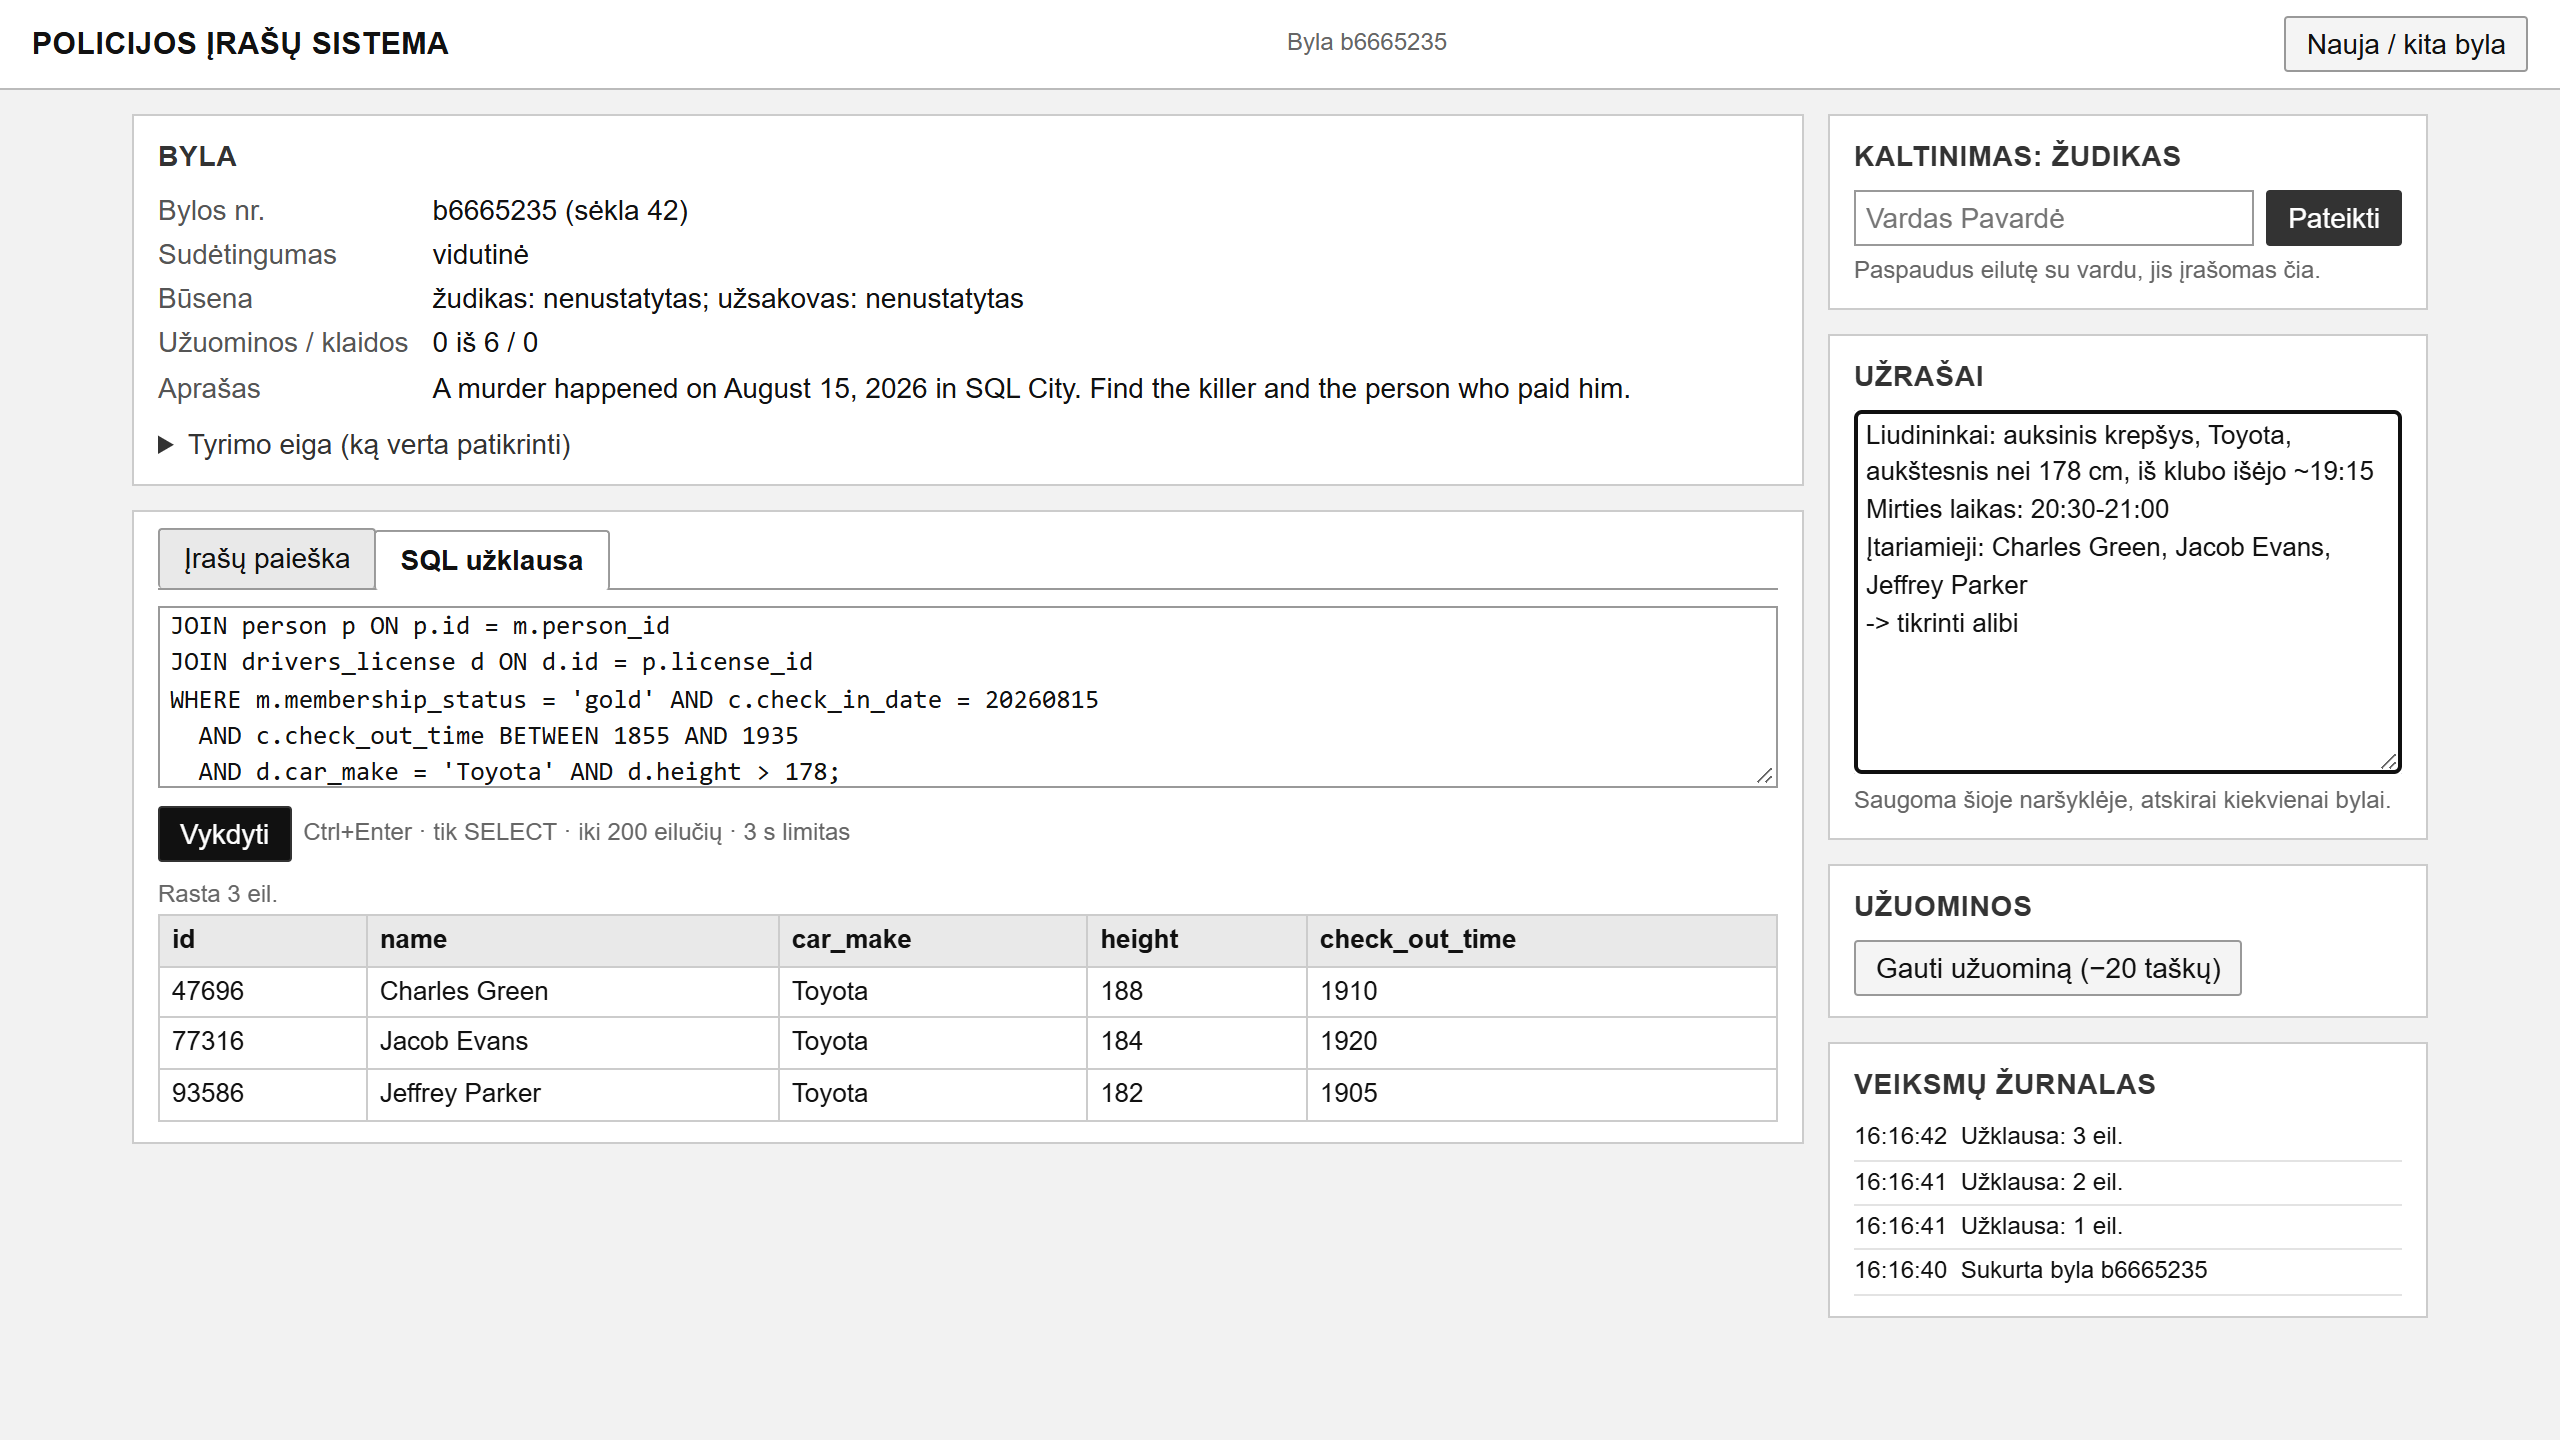
\includegraphics[width=\linewidth, trim=0 260 0 0, clip]{img/web_ui.png}};
    \begin{scope}[x={(img.south east)}, y={(img.north west)}]
        \foreach \n/\x/\y in {1/0.045/0.87, 2/0.06/0.53, 3/0.035/0.29, 4/0.10/0.13,
                              5/0.70/0.87, 6/0.71/0.69, 7/0.71/0.23}
            \node[circle, fill=red!75!black, text=white, font=\tiny\bfseries, inner sep=1.2pt] at (\x,\y) {\n};
    \end{scope}
\end{tikzpicture}
\par\smallskip
{\tiny Atidarymas: \texttt{http://<VM-IP>:8080} (arba vietoje: \texttt{python detective.py setup}, tada \texttt{python web.py}).}
\end{column}

\begin{column}{0.35\textwidth}
\scriptsize
\begin{enumerate}
    \setlength{\itemsep}{1pt}
    \item \textbf{Byla:} pasirinkite lygį (ir sėklą), spauskite „Sukurti naują bylą“. Matote aprašą.
    \item \textbf{Įrašų paieška:} lentelė + sąlygos, be SQL. Arba \textbf{SQL užklausa}.
    \item \textbf{Vykdyti} (Ctrl+Enter). Tik \texttt{SELECT}, iki 200 eil.
    \item \textbf{Rezultatai.} Šalia \texttt{person\_id} rodomas vardas.
    \item \textbf{Kaltinimas:} paspauskite eilutę su vardu, tada „Pateikti“.
    \item \textbf{Užrašai} įtariamiesiems ir alibi.
    \item \textbf{Užuomina} kainuoja 20 taškų.
\end{enumerate}
\end{column}
\end{columns}

\end{frame}

% ============================================================
% 3. PAVYZDYS: BYLA ŽINGSNIS PO ŽINGSNIO
% ============================================================
\begin{frame}{Pavyzdys: byla per 6 užklausas (vidutinė, sėkla 42)}

\scriptsize
\setlength{\tabcolsep}{3pt}
\begin{tabular}{@{}c>{\raggedright\arraybackslash}p{0.14\textwidth}>{\raggedright\arraybackslash}p{0.33\textwidth}>{\raggedright\arraybackslash}p{0.48\textwidth}@{}}
\toprule
\# & Žingsnis & Kur ieškoti & Ką rasite \\
\midrule
1 & Ataskaita & ataskaitos: murder, SQL City, 20260815 & auka, mirties laikas 20:30--21:00, 2 liudininkai \\
2 & Liudininkai & asmenys, apklausos & Toyota, aukštesnis nei 178 cm, auksinis krepšys, 19:15 \\
3 & Įtariamieji & klubas + apsilankymai + pažymėjimai & \textbf{3 vyrai}, ne vienas \\
4 & Alibi & apklausos, renginiai, ataskaitos, klubas & du turi alibi; vienas meluoja apie klubą ir renginį \\
5 & Motyvas & ataskaitos su aukos vardu & muštynės su auka ir vienas klaidinantis įrašas \\
6 & Užsakovė & anoniminis pranešimas + \texttt{GROUP BY} & tik viena moteris atitinka visus požymius \\
\bottomrule
\end{tabular}

\vspace{2mm}
\begin{columns}[T]
\begin{column}{0.50\textwidth}
\begin{block}{Kaip suprasti rezultatus}
\tiny
\begin{itemize}
    \setlength{\itemsep}{0pt}
    \item „Wrong killer“: klaida, $-25$ taškų. „Correct“: kitas etapas.
    \item Taškai: 100 / 250 / 500 pagal lygį, $-20$ už užuominą.
    \item „Įrašų nerasta“: patikrinkite datą (YYYYMMDD) ir rašybą.
\end{itemize}
\end{block}
\end{column}
\begin{column}{0.48\textwidth}
\begin{block}{Turi nepavykti (saugumas)}
\tiny
\texttt{DELETE FROM person}: atmesta\\
\texttt{SELECT * FROM game.cases}: nėra teisių\\
\texttt{SELECT pg\_sleep(10)}: nutraukta po 3 s\\[2pt]
Visos užklausos: \texttt{PTJ\_access\_info.txt}
\end{block}
\end{column}
\end{columns}

\end{frame}

% ============================================================
% 10. IŠŠŪKIAI IR ATEITIES PLANAI
% ============================================================
\begin{frame}{Iššūkiai ir ateities planai}

\begin{columns}[T]
\begin{column}{0.60\textwidth}
\scriptsize
\begin{tabular}{@{}>{\raggedright\arraybackslash}p{0.44\textwidth}>{\raggedright\arraybackslash}p{0.52\textwidth}@{}}
\toprule
\textbf{Problema} & \textbf{Sprendimas} \\
\midrule
Žudikas randamas viena užklausa & Aprašymas tinka keliems, alibi kitose lentelėse, melas ir motyvas \\ \addlinespace[2pt]
Prisipažinimas apklausoje & Užsakovės įkalčiai anoniminiame pranešime \\ \addlinespace[2pt]
Per didelė DB (1955 įrašai) & 477 įrašai, mažas miestas \\ \addlinespace[2pt]
Byla gali turėti kelis sprendinius & SQL patikra, ROLLBACK, kitas bandymas \\ \addlinespace[2pt]
Bendra rolė + \texttt{SET ROLE} & Atskira rolė kiekvienai bylai \\ \addlinespace[2pt]
Sunkios užklausos & 3 s limitas ir \texttt{LIMIT 200} \\
\bottomrule
\end{tabular}
\end{column}

\begin{column}{0.38\textwidth}
\begin{block}{Toliau}
\footnotesize
\begin{itemize}
    \item \textbf{Faker}: įvairesni duomenys.
    \item Daugiau alibi ir motyvų tipų.
    \item Atskiros VM duomenų bazei ir žaidėjams.
    \item Automatinis senų bylų šalinimas.
    \item Rezultatų lentelė.
\end{itemize}
\end{block}
\end{column}
\end{columns}

\vspace{3mm}
\begin{center}
\large Ačiū už dėmesį! Klausimai?
\end{center}

\end{frame}

\end{document}
